\subsection{Discussion}
First of all, it is important to state that we do not view measurement
clusterization as undesirable, nor do we believe it should be avoided
at all. Clusterization is a peculiar phenomenon and it is perfectly
reasonable for someone to argue against the D-optimality criterion
based on the fact that it results in clustered designs. We have seen,
however that there is perfectly reasonable explanation for
clusterization, i.e.~that clusterization arises when we seek a
designWe have shown that clusterization is an innevitable conseqeunce
of having a problem with modes of higher uncertainty than
others. Clusterization manifests the true underlying objective


\subsubsection{Answer to Question \ref{q:why}}
Armed with Theorem \ref{thm:char} we can give a compelling explanation
of the measurement clusterization we obeserved in
Fig.~\ref{fig:}. From part (..) of the Theorem \ref{thm:char} and
Fig.~\ref{fig:tikz clusterization}, we know that a D-optimal design
aims to reduce uncertainty of eigenvectors of
$(\fwd\prcov\fwd^*)^{-1}$ where prior covariance eigenvalues
$\lambda_j$ are highest. D-optimal design will try to focus on the
leading eigenvectors of $(\fwd\prcov\fwd^*)^{-1}$ and take
measurements where other \emph{scaled} eigenvectors are close to
zero.

For concreteness, let us assume that in a certain problem, a D-optimal
design aims to measure only the two leading eigenvectors, i.e.~$\rank
\obs^*\obs =: k=2$. Thus, a D-optimal design will (try to) ignore all
eigenvectors corresponding to $j > 2$. Since $\lambda_j$ decay to
zero, a D-optimal design should only try to avoid eigenvectors for
which $\lambda_j$ is not already small --- e.g.~eigenvectors
$j=3,4$. It is possible that the geometry of the domain $\Omega$ and
the structure of the eigenvectors leave only a few locations in
$\Omega$ where the amplitude of eigenvectors $j=1,2$ is high while the
amplitude of eigenvectors $j=3,4$ is low. In such case, clusterization
will occur whenever the number of measurements $m$ is large enough, by
the pigeonhole principle. This scenario is illustrated for the inverse
problem of the 1D heat equation in Fig.~\ref{fig:eigenvectors}.

\begin{figure}\label{fig:eigenvectors}
    \centering
    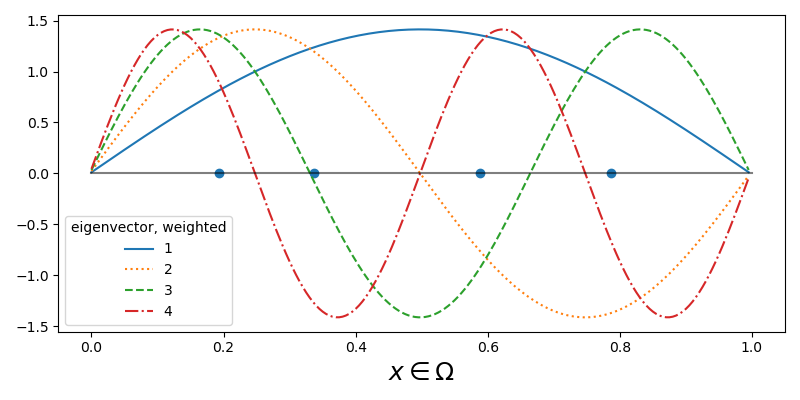
\includegraphics[width=\textwidth]{eigenvectors_dst.pdf}
    \caption{D-optimal measurement locations ($m=4$ measurements) and
      weighted eigenvectors for finding the initial condition of
      the 1D heat equation. Measurement locations and weighted
      eigenvectors are plotted over the computational domain $\Omega =
      [0, 1]$ (x-axis). Measurement clusterization occurs
      approximately at $0.31$ and $0.69$. These two locations are a
      compromise between zeros of eigenvectors a D-optimal design aims
      to ignore (third and up) and staying far from zeros of the
      eigenvectors a D-optimal design aims to measure (first and
      second). Allocating $m=4$ measurements into two locations
      results in clusterization, according to the pigeonhole
      principle.}
  \label{fig:why}
\end{figure}



By Weyl's law, eigenvalues $\lambda_j$ of the Laplace operator
increase as $\lambda_j \sim j^{d/2}$, where $d = \dim \Omega$ is the
dimensionality of the domain. In accordance with Weyl's law,
\cite[Theorem 3.1]{Stuart10} suggests taking priors as
"Laplacian-like" operators to power smaller than $-\frac{d}{2}$, to
maintain regularity of posterior realizations. Thus, even though the
computational domain is getting larger and sparser as the dimension
$d$ grows, clusterization is not necessarily harder to achieve.

%% In our model we did not specify any specific prior, so it is possible
%% that one will be able to devise a prior that will not result in
%% clusterization. Indeed, if the rate of increase of prior precision
%% eigenvalues is small, 


As mentioned in the Limitations section, our model does not accomodate
point evaluations. For example, in the inverse problem of the 1D heat
equation, it seems reasonable to take $\hilp = \hilo =
L^2(\Omega)$. Unfortunately, for any point evaluation $\delta_x \not
\in L^2(\Omega)$.are taken of the final heat distribution $u_T$. If we
consider the initial and final conditions $u_0$ and $u_T$ as elements
of $L^2([0,1])$, theheat equation as
